
%% bare_jrnl_transmag.tex
%% V1.4
%% 2012/12/27
%% by Michael Shell
%% see http://www.michaelshell.org/
%% for current contact information.
%%
%% This is a skeleton file demonstrating the use of IEEEtran.cls
%% (requires IEEEtran.cls version 1.8 or later) with an IEEE 
%% Transactions on Magnetics journal paper.
%%
%% Support sites:
%% http://www.michaelshell.org/tex/ieeetran/
%% http://www.ctan.org/tex-archive/macros/latex/contrib/IEEEtran/
%% and
%% http://www.ieee.org/



% *** Authors should verify (and, if needed, correct) their LaTeX system  ***
% *** with the testflow diagnostic prior to trusting their LaTeX platform ***
% *** with production work. IEEE's font choices can trigger bugs that do  ***
% *** not appear when using other class files.                            ***
% The testflow support page is at:
% http://www.michaelshell.org/tex/testflow/


%%*************************************************************************
%% Legal Notice:
%% This code is offered as-is without any warranty either expressed or
%% implied; without even the implied warranty of MERCHANTABILITY or
%% FITNESS FOR A PARTICULAR PURPOSE! 
%% User assumes all risk.
%% In no event shall IEEE or any contributor to this code be liable for
%% any damages or losses, including, but not limited to, incidental,
%% consequential, or any other damages, resulting from the use or misuse
%% of any information contained here.
%%
%% All comments are the opinions of their respective authors and are not
%% necessarily endorsed by the IEEE.
%%
%% This work is distributed under the LaTeX Project Public License (LPPL)
%% ( http://www.latex-project.org/ ) version 1.3, and may be freely used,
%% distributed and modified. A copy of the LPPL, version 1.3, is included
%% in the base LaTeX documentation of all distributions of LaTeX released
%% 2003/12/01 or later.
%% Retain all contribution notices and credits.
%% ** Modified files should be clearly indicated as such, including  **
%% ** renaming them and changing author support contact information. **
%%
%% File list of work: IEEEtran.cls, IEEEtran_HOWTO.pdf, bare_adv.tex,
%%                    bare_conf.tex, bare_jrnl.tex, bare_jrnl_compsoc.tex,
%%                    bare_jrnl_transmag.tex
%%*************************************************************************

% Note that the a4paper option is mainly intended so that authors in
% countries using A4 can easily print to A4 and see how their papers will
% look in print - the typesetting of the document will not typically be
% affected with changes in paper size (but the bottom and side margins will).
% Use the testflow package mentioned above to verify correct handling of
% both paper sizes by the user's LaTeX system.
%
% Also note that the "draftcls" or "draftclsnofoot", not "draft", option
% should be used if it is desired that the figures are to be displayed in
% draft mode.
%
\documentclass[journal]{IEEEtran}
%
% If IEEEtran.cls has not been installed into the LaTeX system files,
% manually specify the path to it like:
% \documentclass[journal]{../sty/IEEEtran}





% Some very useful LaTeX packages include:
% (uncomment the ones you want to load)


% *** MISC UTILITY PACKAGES ***
%
%\usepackage{ifpdf}
% Heiko Oberdiek's ifpdf.sty is very useful if you need conditional
% compilation based on whether the output is pdf or dvi.
% usage:
% \ifpdf
%   % pdf code
% \else
%   % dvi code
% \fi
% The latest version of ifpdf.sty can be obtained from:
% http://www.ctan.org/tex-archive/macros/latex/contrib/oberdiek/
% Also, note that IEEEtran.cls V1.7 and later provides a builtin
% \ifCLASSINFOpdf conditional that works the same way.
% When switching from latex to pdflatex and vice-versa, the compiler may
% have to be run twice to clear warning/error messages.






% *** CITATION PACKAGES ***
%
%\usepackage{cite}
% cite.sty was written by Donald Arseneau
% V1.6 and later of IEEEtran pre-defines the format of the cite.sty package
% \cite{} output to follow that of IEEE. Loading the cite package will
% result in citation numbers being automatically sorted and properly
% "compressed/ranged". e.g., [1], [9], [2], [7], [5], [6] without using
% cite.sty will become [1], [2], [5]--[7], [9] using cite.sty. cite.sty's
% \cite will automatically add leading space, if needed. Use cite.sty's
% noadjust option (cite.sty V3.8 and later) if you want to turn this off
% such as if a citation ever needs to be enclosed in parenthesis.
% cite.sty is already installed on most LaTeX systems. Be sure and use
% version 4.0 (2003-05-27) and later if using hyperref.sty. cite.sty does
% not currently provide for hyperlinked citations.
% The latest version can be obtained at:
% http://www.ctan.org/tex-archive/macros/latex/contrib/cite/
% The documentation is contained in the cite.sty file itself.






% *** GRAPHICS RELATED PACKAGES ***
%
\ifCLASSINFOpdf
  % \usepackage[pdftex]{graphicx}
  % declare the path(s) where your graphic files are
  % \graphicspath{{../pdf/}{../jpeg/}}
  % and their extensions so you won't have to specify these with
  % every instance of \includegraphics
  % \DeclareGraphicsExtensions{.pdf,.jpeg,.png}
\else
  % or other class option (dvipsone, dvipdf, if not using dvips). graphicx
  % will default to the driver specified in the system graphics.cfg if no
  % driver is specified.
  % \usepackage[dvips]{graphicx}
  % declare the path(s) where your graphic files are
  % \graphicspath{{../eps/}}
  % and their extensions so you won't have to specify these with
  % every instance of \includegraphics
  % \DeclareGraphicsExtensions{.eps}
\fi
% graphicx was written by David Carlisle and Sebastian Rahtz. It is
% required if you want graphics, photos, etc. graphicx.sty is already
% installed on most LaTeX systems. The latest version and documentation
% can be obtained at: 
% http://www.ctan.org/tex-archive/macros/latex/required/graphics/
% Another good source of documentation is "Using Imported Graphics in
% LaTeX2e" by Keith Reckdahl which can be found at:
% http://www.ctan.org/tex-archive/info/epslatex/
%
% latex, and pdflatex in dvi mode, support graphics in encapsulated
% postscript (.eps) format. pdflatex in pdf mode supports graphics
% in .pdf, .jpeg, .png and .mps (metapost) formats. Users should ensure
% that all non-photo figures use a vector format (.eps, .pdf, .mps) and
% not a bitmapped formats (.jpeg, .png). IEEE frowns on bitmapped formats
% which can result in "jaggedy"/blurry rendering of lines and letters as
% well as large increases in file sizes.
%
% You can find documentation about the pdfTeX application at:
% http://www.tug.org/applications/pdftex




% *** MATH PACKAGES ***
%
%\usepackage[cmex10]{amsmath}
% A popular package from the American Mathematical Society that provides
% many useful and powerful commands for dealing with mathematics. If using
% it, be sure to load this package with the cmex10 option to ensure that
% only type 1 fonts will utilized at all point sizes. Without this option,
% it is possible that some math symbols, particularly those within
% footnotes, will be rendered in bitmap form which will result in a
% document that can not be IEEE Xplore compliant!
%
% Also, note that the amsmath package sets \interdisplaylinepenalty to 10000
% thus preventing page breaks from occurring within multiline equations. Use:
%\interdisplaylinepenalty=2500
% after loading amsmath to restore such page breaks as IEEEtran.cls normally
% does. amsmath.sty is already installed on most LaTeX systems. The latest
% version and documentation can be obtained at:
% http://www.ctan.org/tex-archive/macros/latex/required/amslatex/math/





% *** SPECIALIZED LIST PACKAGES ***
%
%\usepackage{algorithmic}
% algorithmic.sty was written by Peter Williams and Rogerio Brito.
% This package provides an algorithmic environment fo describing algorithms.
% You can use the algorithmic environment in-text or within a figure
% environment to provide for a floating algorithm. Do NOT use the algorithm
% floating environment provided by algorithm.sty (by the same authors) or
% algorithm2e.sty (by Christophe Fiorio) as IEEE does not use dedicated
% algorithm float types and packages that provide these will not provide
% correct IEEE style captions. The latest version and documentation of
% algorithmic.sty can be obtained at:
% http://www.ctan.org/tex-archive/macros/latex/contrib/algorithms/
% There is also a support site at:
% http://algorithms.berlios.de/index.html
% Also of interest may be the (relatively newer and more customizable)
% algorithmicx.sty package by Szasz Janos:
% http://www.ctan.org/tex-archive/macros/latex/contrib/algorithmicx/




% *** ALIGNMENT PACKAGES ***
%
%\usepackage{array}
% Frank Mittelbach's and David Carlisle's array.sty patches and improves
% the standard LaTeX2e array and tabular environments to provide better
% appearance and additional user controls. As the default LaTeX2e table
% generation code is lacking to the point of almost being broken with
% respect to the quality of the end results, all users are strongly
% advised to use an enhanced (at the very least that provided by array.sty)
% set of table tools. array.sty is already installed on most systems. The
% latest version and documentation can be obtained at:
% http://www.ctan.org/tex-archive/macros/latex/required/tools/


% IEEEtran contains the IEEEeqnarray family of commands that can be used to
% generate multiline equations as well as matrices, tables, etc., of high
% quality.




% *** SUBFIGURE PACKAGES ***
%\ifCLASSOPTIONcompsoc
%  \usepackage[caption=false,font=normalsize,labelfont=sf,textfont=sf]{subfig}
%\else
%  \usepackage[caption=false,font=footnotesize]{subfig}
%\fi
% subfig.sty, written by Steven Douglas Cochran, is the modern replacement
% for subfigure.sty, the latter of which is no longer maintained and is
% incompatible with some LaTeX packages including fixltx2e. However,
% subfig.sty requires and automatically loads Axel Sommerfeldt's caption.sty
% which will override IEEEtran.cls' handling of captions and this will result
% in non-IEEE style figure/table captions. To prevent this problem, be sure
% and invoke subfig.sty's "caption=false" package option (available since
% subfig.sty version 1.3, 2005/06/28) as this is will preserve IEEEtran.cls
% handling of captions.
% Note that the Computer Society format requires a larger sans serif font
% than the serif footnote size font used in traditional IEEE formatting
% and thus the need to invoke different subfig.sty package options depending
% on whether compsoc mode has been enabled.
%
% The latest version and documentation of subfig.sty can be obtained at:
% http://www.ctan.org/tex-archive/macros/latex/contrib/subfig/



% *** FLOAT PACKAGES ***
%
%\usepackage{fixltx2e}
% fixltx2e, the successor to the earlier fix2col.sty, was written by
% Frank Mittelbach and David Carlisle. This package corrects a few problems
% in the LaTeX2e kernel, the most notable of which is that in current
% LaTeX2e releases, the ordering of single and double column floats is not
% guaranteed to be preserved. Thus, an unpatched LaTeX2e can allow a
% single column figure to be placed prior to an earlier double column
% figure. The latest version and documentation can be found at:
% http://www.ctan.org/tex-archive/macros/latex/base/


%\usepackage{stfloats}
% stfloats.sty was written by Sigitas Tolusis. This package gives LaTeX2e
% the ability to do double column floats at the bottom of the page as well
% as the top. (e.g., "\begin{figure*}[!b]" is not normally possible in
% LaTeX2e). It also provides a command:
%\fnbelowfloat
% to enable the placement of footnotes below bottom floats (the standard
% LaTeX2e kernel puts them above bottom floats). This is an invasive package
% which rewrites many portions of the LaTeX2e float routines. It may not work
% with other packages that modify the LaTeX2e float routines. The latest
% version and documentation can be obtained at:
% http://www.ctan.org/tex-archive/macros/latex/contrib/sttools/
% Do not use the stfloats baselinefloat ability as IEEE does not allow
% \baselineskip to stretch. Authors submitting work to the IEEE should note
% that IEEE rarely uses double column equations and that authors should try
% to avoid such use. Do not be tempted to use the cuted.sty or midfloat.sty
% packages (also by Sigitas Tolusis) as IEEE does not format its papers in
% such ways.
% Do not attempt to use stfloats with fixltx2e as they are incompatible.
% Instead, use Morten Hogholm'a dblfloatfix which combines the features
% of both fixltx2e and stfloats:
%
% \usepackage{dblfloatfix}
% The latest version can be found at:
% http://www.ctan.org/tex-archive/macros/latex/contrib/dblfloatfix/




%\ifCLASSOPTIONcaptionsoff
%  \usepackage[nomarkers]{endfloat}
% \let\MYoriglatexcaption\caption
% \renewcommand{\caption}[2][\relax]{\MYoriglatexcaption[#2]{#2}}
%\fi
% endfloat.sty was written by James Darrell McCauley, Jeff Goldberg and 
% Axel Sommerfeldt. This package may be useful when used in conjunction with 
% IEEEtran.cls'  captionsoff option. Some IEEE journals/societies require that
% submissions have lists of figures/tables at the end of the paper and that
% figures/tables without any captions are placed on a page by themselves at
% the end of the document. If needed, the draftcls IEEEtran class option or
% \CLASSINPUTbaselinestretch interface can be used to increase the line
% spacing as well. Be sure and use the nomarkers option of endfloat to
% prevent endfloat from "marking" where the figures would have been placed
% in the text. The two hack lines of code above are a slight modification of
% that suggested by in the endfloat docs (section 8.4.1) to ensure that
% the full captions always appear in the list of figures/tables - even if
% the user used the short optional argument of \caption[]{}.
% IEEE papers do not typically make use of \caption[]'s optional argument,
% so this should not be an issue. A similar trick can be used to disable
% captions of packages such as subfig.sty that lack options to turn off
% the subcaptions:
% For subfig.sty:
% \let\MYorigsubfloat\subfloat
% \renewcommand{\subfloat}[2][\relax]{\MYorigsubfloat[]{#2}}
% However, the above trick will not work if both optional arguments of
% the \subfloat command are used. Furthermore, there needs to be a
% description of each subfigure *somewhere* and endfloat does not add
% subfigure captions to its list of figures. Thus, the best approach is to
% avoid the use of subfigure captions (many IEEE journals avoid them anyway)
% and instead reference/explain all the subfigures within the main caption.
% The latest version of endfloat.sty and its documentation can obtained at:
% http://www.ctan.org/tex-archive/macros/latex/contrib/endfloat/
%
% The IEEEtran \ifCLASSOPTIONcaptionsoff conditional can also be used
% later in the document, say, to conditionally put the References on a 
% page by themselves.









% *** Do not adjust lengths that control margins, column widths, etc. ***
% *** Do not use packages that alter fonts (such as pslatex).         ***
% There should be no need to do such things with IEEEtran.cls V1.6 and later.
% (Unless specifically asked to do so by the journal or conference you plan
% to submit to, of course. )


% correct bad hyphenation here
\hyphenation{op-tical net-works semi-conduc-tor}
\usepackage{graphicx}
\usepackage{subfloat}
\usepackage{subfigure}
\usepackage{subfig}
\usepackage{color}
\usepackage{amsmath}
\usepackage{amsfonts}
\usepackage{amssymb}
\usepackage{multirow}
\usepackage{algorithm}
\usepackage{algorithmicx}
\usepackage{algpseudocode}
\usepackage{amsmath}
\usepackage{graphics}
\usepackage{epsfig}
\usepackage{CJK}
\usepackage{amsmath}
\usepackage{caption}





\usepackage[font=small,labelsep=period]{caption}
\captionsetup{%
  figurename=Fig.,
  tablename=Table
  }

\begin{document}
%
% paper title
% can use linebreaks \\ within to get better formatting as desired
% Do not put math or special symbols in the title.
\title{Task-Oriented Visual Servo System of Robot Arm for 3D Object based on Automatic Multilayer Networks Learning Approach }



% author names and affiliations
% transmag papers use the long conference author name format.

\author{\IEEEauthorblockN{Ren C. Luo\IEEEauthorrefmark{1},
and Po-Yu Chuang\IEEEauthorrefmark{2},
}

\IEEEauthorblockA{\IEEEauthorrefmark{1} \IEEEauthorrefmark{2}Electrical Engineering Department, National
Taiwan University, Taipei, Taiwan 106}

% <-this % stops an unwanted space
%\thanks{Manuscript received December 1, 2012; revised December %27, 2012. 
%Corresponding author: M. Shell (email: http://%www.michaelshell.org/contact.html).}
}



% The paper headers
%\markboth{Journal of \LaTeX\ Class Files,~Vol.~11, No.~4, December~2012}%
%{Shell \MakeLowercase{\textit{et al.}}: Bare Demo of IEEEtran.cls for Journals}
% The only time the second header will appear is for the odd numbered pages
% after the title page when using the twoside option.
% 
% *** Note that you probably will NOT want to include the author's ***
% *** name in the headers of peer review papers.                   ***
% You can use \ifCLASSOPTIONpeerreview for conditional compilation here if
% you desire.




% If you want to put a publisher's ID mark on the page you can do it like
% this:
%\IEEEpubid{0000--0000/00\$00.00~\copyright~2012 IEEE}
% Remember, if you use this you must call \IEEEpubidadjcol in the second
% column for its text to clear the IEEEpubid mark.



% use for special paper notices
%\IEEEspecialpapernotice{(Invited Paper)}


% for Transactions on Magnetics papers, we must declare the abstract and
% index terms PRIOR to the title within the \IEEEtitleabstractindextext
% IEEEtran command as these need to go into the title area created by
% \maketitle.
% As a general rule, do not put math, specaial symbols or citations
% in the abstract or keywords.
\IEEEtitleabstractindextext{%
\begin{abstract}
Visual servo systems are widely applied on industrial robot arm recent years. A visual servo system could provide additional perception of robot arm, and make it more robust in different applications. In this paper, we propose an intelligent visual servo system which could automatically learn the model of unknown 3D objects, and self-supervised the results. Unlike traditional vision-based learning approaches, proposed learning system is task-oriented which means learning approaches only concern the relation between input and target rather then each individual part. To construct connections between input and target,the learning approach is established based on multi-layers networks. Multi-layers networks is used to model necessary knowledges in different domains.  The experiment results show the feasibility of proposed structure for automatic learning, and multi-layers networks could effectively transfer knowledge between different domains.
\end{abstract}

% Note that keywords are not normally used for peerreview papers.
\begin{IEEEkeywords}
Visual servo system, Multi-layers network, Machine learning
\end{IEEEkeywords}}



% make the title area
\maketitle


% To allow for easy dual compilation without having to reenter the
% abstract/keywords data, the \IEEEtitleabstractindextext text will
% not be used in maketitle, but will appear (i.e., to be "transported")
% here as \IEEEdisplaynontitleabstractindextext when the compsoc 
% or transmag modes are not selected <OR> if conference mode is selected 
% - because all conference papers position the abstract like regular
% papers do.
\IEEEdisplaynontitleabstractindextext
% \IEEEdisplaynontitleabstractindextext has no effect when using
% compsoc or transmag under a non-conference mode.







% For peer review papers, you can put extra information on the cover
% page as needed:
% \ifCLASSOPTIONpeerreview
% \begin{center} \bfseries EDICS Category: 3-BBND \end{center}
% \fi
%
% For peerreview papers, this IEEEtran command inserts a page break and
% creates the second title. It will be ignored for other modes.
\IEEEpeerreviewmaketitle



\section{Introduction}


% The very first letter is a 2 line initial drop letter followed
% by the rest of the first word in caps.
% 
% form to use if the first word consists of a single letter:
% \IEEEPARstart{A}{demo} file is ....
% 
% form to use if you need the single drop letter followed by
% normal text (unknown if ever used by IEEE):
% \IEEEPARstart{A}{}demo file is ....
% 
% Some journals put the first two words in caps:
% \IEEEPARstart{T}{his demo} file is ....
% 
% Here we have the typical use of a "T" for an initial drop letter
% and "HIS" in caps to complete the first word.
\IEEEPARstart{R}{obot} arm with visual servo system had been widely applied in automatic industrial production line recent years[1]. Visual servo system provides additional perception of environment, and make robot arm become more adaptive to complete various tasks. The visual servo based robot arm systems are generally divided into two parts in previous works [2-4]. One is vision system which is used to detect or track targets, and estimate the states of targets for robot arm. The other is robot arm which could use received states and execute pre-programmed scenario to complete tasks. Although many present works is already robust enough for real practice, there are still some issues have to be concurred. 

For vision system, model-based recognition methods are commonly used in industrial application. Model-based methods are famous for efficiency and robustness. The performance is mainly related to the input data which is captured manually. Hence, the system is hard to adapt with the changing of work pieces, manufactured processing,etc. For 2D object recognition, users need to capture numerous raw data of target objects in specific poses. These cumbersome works would become much more complex while the methods are expanded to 3D object recognition. Even though the states of objects had been precisely estimated, the states have to be further transformed to the coordination of robot. The coefficients of coordinate transformation also have to be manually adjusted depend on different cases. These manual works not only increase the labor cost, but also point out the dilemma of present vision-based robot which is unable to automatically adapt to various assignments. To solve these issues,we propose an intelligent tasked-oriented visual servo based system which can automatically learn image models of targets, and able to self-refine the relative function of input and target.

In general industrial purposes, we do not really concern about all details of entire target. Instead, the relation between input and target is the key point for completing the tasks like pick and place, work pieces arrangement, components insertion,etc. Take pick and place as an example, in task-oriented view, system tends to manipulate robot arm to pick work pieces and place them in specific pose. Therefore, proposed system focus on constructing relation between input images and rotation angles of robot arm, rather than a delicate 3-D object model. The input of system is 2-D image data, and output is rotation angle of robot arm in Cartesian space. Unfortunately, the input and output are different feature domains(image space to Cartesian space), so the traditional single model learning approach[5] is not enough to solve our problem.

The features in different domains can be quantified and integrated into multilayer networks.  The most well-known multilayer networks are multilayer perceptron (MLP). MLP is feed forward neural networks with multiple layers neurons. Although MLP had been well studied and enable to apply in a wide variety of research field, MLP requires input and output is in the same domains such as feature to feature, or object to object. Hence, we propose a new multilayer networks structure which tends to integrate different level’s information, and further infer the relationship between different domains. The distribution of different domains is not possible the same, and also hard to be modelled through limited data. Therefore, the learning of different domains have to be relied on transfer learning[6-9]. Transfer learning methods are arise while source domain and target domain are different or data is easily outdated[13]. In our case, the network is composed by three different domains: image, object and Cartesian space. To integrate three domains into one network, we build relative functions between each domain for mapping the information between different domains. The parameters of relative functions are able to be refined through proposed transfer learning approach. 
 
%%%%%Revised to here%%%%%%%%%%%%%%%
In proposed system, the final poses of target objects are essential prior of proposed system, because final poses would be different dependent on different requirements. For a 3-D objects, this prior only provides information of target face, but other faces are unknown. Hence, building a descriptor which can be used to infer the relations of input and target poses is necessary. Constructing descriptor of object is a pervasive topic in areas of computer vision, and there are many brilliant existed approaches with high quality and low computation cost [10-14]. Most of these methods are focus on building descriptor from strong sparse features in input image. The sparse features are selected based on designed approaches, and weak feature points would be wiped out. Therefore, some information might lose in selecting process. Different faces of the same object might derive different strong feature points, so more information is needed for inferring relation in our issue. Instead of choosing sparse features, uniform distributed feature is more suitable for finding obscure co-features in different viewpoints. Unfortunately, uniform distributed feature such as RGB and texture are easily affected by environment, and these uncertainties would reduce the robustness of descriptors.  

To conquer the uncertainties of low-level feature, we proposed a descriptor which is constructed based on Markov Logic Network (MLN) [15]. MLN is an approach combines first-order logic and probabilistic graphical model. Probabilistic graphical models are famous for handling uncertainty. First-order logic enable compactly representing a wide variety of knowledge, and widely applied on statistical relational learning [16-18].  Therefore, MLN is used to describe the structure of an object in different view-point (image domain), and build 2-D descriptors which are constructed by first-order logic formulas. MLN-based descriptors could be further applied to connect the relation between different faces of the same object by matching co-features. The relational model of 3-D object is consisted by multiple 2-D descriptors, and is represented by vector in Cartesian Space. Therefore, the relational model is not only integrate 2-D descriptors into 3-D object, but also utilize to derive rotation angle of robot arm through vector in Cartesian Space. By doing so, the relation between input and target could be established, and help robot arm to complete assign task.  

In this paper,we start with briefly overview of system design and structure in section 2. The MLN-based descriptor for recognized object would be revealed in section 3. Section 4 introduces how to model the proposed multilayer networks, and build up and refine the structure of databased for matching. Then, we compare the performance of proposed system with several different features and descriptors in section 5. Finally, the performance review and conclusion would be discussed in final section.

\begin{figure}[!t]
\begin{center}
%\subfigure[System architecture]{}
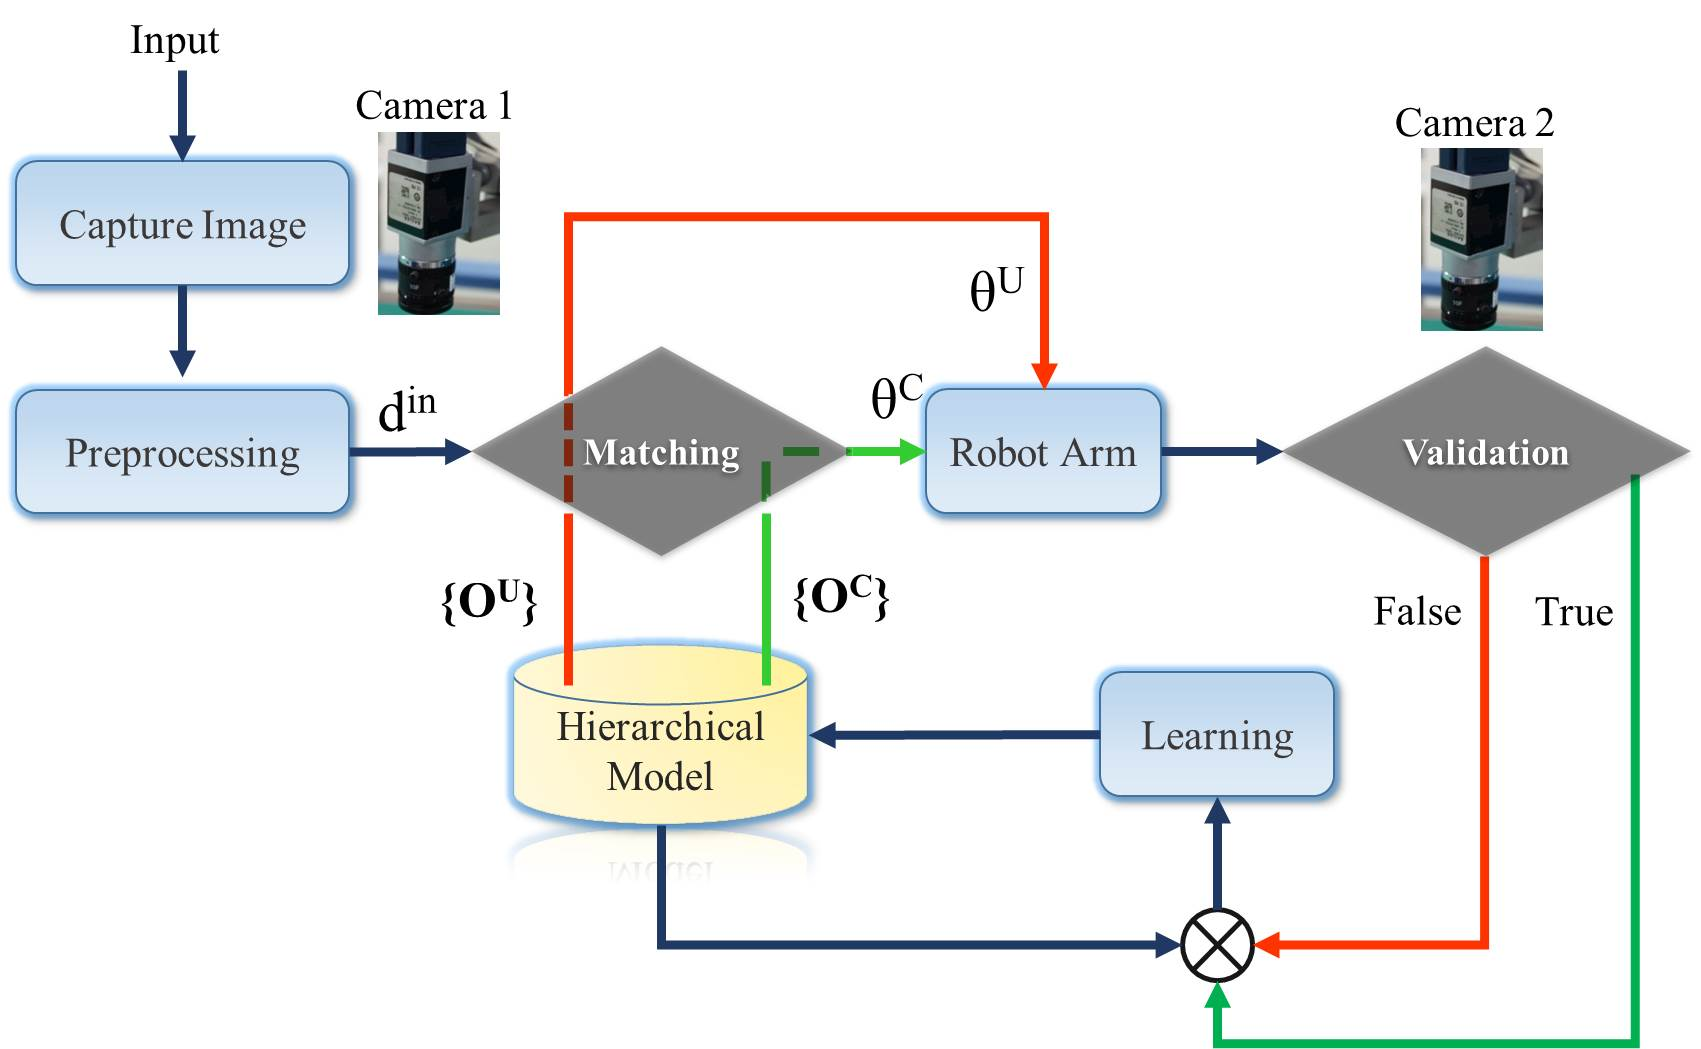
\includegraphics[width=0.5\textwidth]{j_img/fig1.jpg}
\caption{System architecture}\label{test}
\end{center}
\end{figure}




%\hfill mds
\section{System architecture} 
The main purpose of this system is that desire to automatically derive the orientation relationship between input poses and target poses without 3-D model of input objects, and guide robot arm to pick and complete assigned tasks. The target poses of work pieces have to be given by users. Users then only need to put the work pieces on the conveyor arbitrarily, and the relationship would be learned by proposed approach automatically. This system is consisted by three main parts: Firstly, camera 1 in fig. 1 capture all input work pieces with arbitrary poses, and classify the features of each single work piece through clustering or segmentation method [19-23]. For each work piece, camera 1 would capture serial images while work pieces move into FOV as shown in fig. 2(a). The descriptors of every input work pieces would be constructed by these serial images. Hereafter, system would search matched descriptors from database, and guide robot arm to pick the work pieces and rotate to target pose. Otherwise, the system would infer the most possible result through proposed method, and guide robot arm to pick works pieces based on inferred results. 

\begin{figure}[!t]
\begin{center}
\subfigure[Serial captured frames]{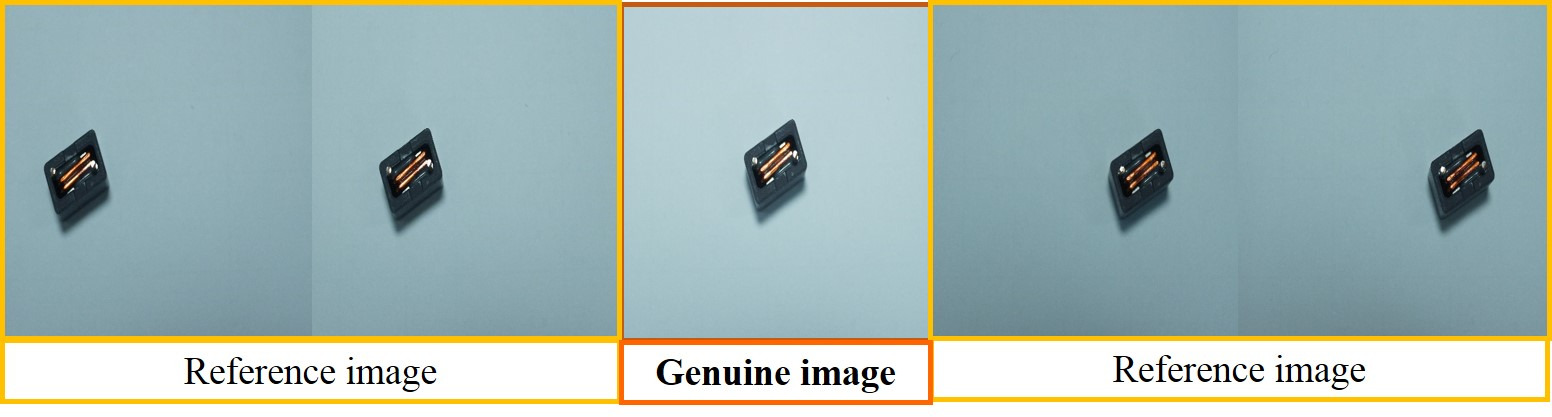
\includegraphics[width=3.5in]{j_img/fig2a.jpg}}
\subfigure[Result of background subtracting and clustering]{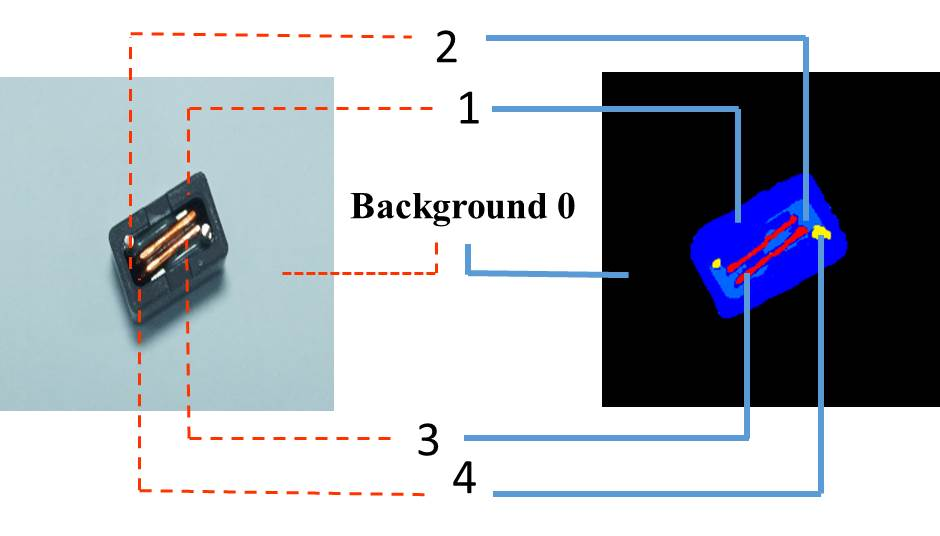
\includegraphics[width=2.5in]{j_img/fig2b.jpg}}
\caption{Preprocessing of input objects}\label{test}
\end{center}
\end{figure}


\begin{figure*}[!t]
\begin{center}
%\subfigure[System architecture]{}
\includegraphics*[width=5 in]{j_img/fig3.jpg}
\caption{Example flow of variables in multi-layers networks}\label{test}
\end{center}
\end{figure*}

For the second part of system, camera 2 plays a role as supervisor of learning. The results would be labelled as true or false. The constructed descriptors with labels become the input of multilayer networks. The third part is learning approach of multilayer networks. The labelled data would be added to the networks after each cycle of system. The labels are used to refine the training result of multilayer networks. Based on these three parts, this system can automatically learn the relative model for robot arm to complete tasks without any manual operation. 

The variables of our model can be classified into six types:

\begin{displaymath}
\{\bf{\Gamma},\bf{D^{in}},\bf{O^{{C}}},\bf{O^{{U}}},\bf{D^{C}_{m}},\bf{D^{U}_{n},\bf{\Theta}}\}
\end{displaymath}

The relation between each variable is illustrated in fig. 3. $\Gamma$ is a set of object 1 to W from camera 1 in feature domain. $\bf{\Gamma_w}$  is a set of serial captured frames of an object w, which is composited by genuine and reference images in fig. 2. $\Gamma_{wg}$ is the genuine image, and $\Gamma_{wn}$ is number $n$ reference frames. $\bf{D^{in}}$ is constructed by $\bf{\Gamma}$ based on proposed 2-D descriptor-constructing method in section 3. Descriptor $d^{in}_w$ would be classified to identified object($\bf{O^C}$) or unidentified object ($\bf{O^U}$) based on Most Probable Explanation (MPE). In fig.3, $d^{in}_1$ is delivered to identified object set $\bf{O^C}$. the system would further assign $d^{in}_1$ to the most possible belonging object $\bf{O^C_m}$. Since a 3-D is composed by multiple 2-D images, one object in our system is defined by multiple 2-D descriptors. $\bf{O^C_m}$ is a set of 2-D descriptors of object m. $d^{in}_1$ is considered as new input data of most possible descriptor couple $d^C_{mb}$ in fig.3. Each descriptor couple includes the rotation angle information between input pose (based on 2-D descriptor) and target pose. $\theta^C_{mb}$ is the rotation angle which can make robot arm rotate object m from input to target pose. The result would be checked by camera 2. If it is true, the result is considered as positive evidence, and merged to the learning process. Otherwise, the result is negative evidence.  

Similarly, $d^{in}_2$ is assigned to the unidentified set $\bf{O^U}$. Unidentified set $\bf{O^U}$ is a set of descriptors which hadn't identified the rotation angle of target prior pose. For unidentified $\bf{O^U}$, the system would infer the possible rotation angle $\theta_{inference}$ for input descriptor. The result would be supervised by camera 2. If result is true, the descriptor would be delivered to the identified object set $\bf{O^C}$ as a new discovered face of corresponding object. Otherwise, the descriptor would feedback to unidentified object set $\bf{O^U}$, and record the inference result to avoid the same fail predication. By doing so, the system is ensured to be converged, and all objects could be identified if the input is sufficient enough.

\section{MLN-based Descriptor}
\subsection{The concept of constructing MLN-based descriptor}
Being an automatically system, deriving more valuable information from raw data could help system deriving exact result, and adapt to numerous suspected input. Most of present image descriptors [10-14] are constructed based on strong extracted feature, because strong sparse feature points are consistent even in different environment. Although these kind of descriptors could efficiently and precisely match given object, the descriptors could not suit for cases which need to infer the relation between existing and unknown data. The sparse feature based descriptor would purge weak feature points of input face, but purged points might be valuable for inferring unknown input from existing data. Hence, the descriptor not only need to be robustness, but also provide sufficient information for constructing relationship. The normal distributed features are compact with our requirement which could provide all detail information of input image. Unfortunately, the normal distributed features such as  RGB, HSV, edges, etc. are easily affected by environment. The segmented or clustering results might be different even two images belonging the same object, so the segmented results are hard to match with each other directly. 

Considering the uncertainties of clustering results of normal distributed features, probabilistic model is the best choice for conquering uncertainties. Although there are several attributes changed due to environment effect (e.g. size of clusters), most of geometric relations between each cluster are relative robustness. We desire to construct the probabilistic-based model in MLN by relations between clusters. Segmented results are used to proposed MLN-based descriptor. The main concept of MLN is that use weighted feature function to soft the hard constrains of first-order logic formulas. If a world violate one formula, it become less possible but not impossible. Take our case as example, when a clustering result of image capture by camera 1 have several clusters different from the result in repository, the MLN-based descriptor would only reduce the probability of candidate rather than wipe out of consideration. Hence, probability-based descriptor has more uncertainty tolerance than the other descriptors which are only modelled by the structure of key feature points. 

Markov logic network L is a set of pairs $(F_i, W_i)$, where $F_i$ is a feature function of first-order logic and $W_i$ is weighting of corresponding formula. The first-order logic formulas converted to $\bf{clause form}$ (also known as $\bf{Conjuctive\quad Nornal\quad Form\quad CNF}$) Each node in L means one feature of each feature function $F_i$. The value of $F_i$ is 1 if formula is true and 0 otherwise. The MLN aim to model the joint distribution of a set of variables $\bf{\Gamma_w}=\{\Gamma_{wg},\Gamma_{w1},\Gamma_{w2},\dots,\Gamma_{wN_w}\}$ in fig.3. The genuine image $\Gamma_{wg}$ is the image which center of object is closest to center of camera, so  genuine image could be considered as most representative 2-D face of a 3-D object in serial frames. The probability distribution of $\Gamma_wg$ over possible world $\Gamma_w$ specified by MLN is given by:
\begin{displaymath}
P(\bf{D^{in}=d^{in}_g})=P(\bf{\Gamma_w}=\Gamma_{wg})=\frac{1}{Z}exp(\sum_{i=1}^Fw_in_i(\Gamma_{wg}))
\end{displaymath}
\begin{equation}
\bf{Z}=\sum_{\Gamma_{wn}\in\bf{\Gamma_w}}exp(\sum_{i=1}w_in_i(\Gamma_{wn}))
\end{equation}

Where $\bf{F}$ is number of formulas in $\Gamma_{wn}$ and $n_i(\Gamma_wg)$ is number of grounding of true grounding of $\bf{F_i}$ in $\Gamma_{wg}$.

For proposed MLN-based descriptor, the first order logic are consisted by conjunction form of predicates. Predicate $ne(s_j,s_{neighbor})$ is used to represent the conjunctive neighbours of each clusters. We consider cluster $s_j$ as key atom and sample conjunctive neighbour $s_{neighbour}$ to derive predicate. Each center atom acquire one formula. Therefore, if an object is segmented to $\bf{J}$ kinds of segmented features, it descriptor would would be constructed by $\bf{J}$ firs-order formulas. 

Based on this concept, the MLN-based descriptor could be constructed by following process: The background of input image are subtracted through MOG [21](supported  by open source library OpenCV), and each isolated object is clustered according to RGB features. RGB features are classified into 4 parts for each channel through K-means clustering [22], so the max size N of feature S is 64 in this paper. N can be adjusted dependent on selected clustering method. Fig. 2(b) shows the background subtracted result of genuine image of fig. 2(a), and different classes of feature are labelled different number such as fig. 2(b). The black part means subtracted background and is label 0. The other label number is between 1 and N. Then, taking fig. 2(b) as example, the object is segmented to 4 kinds of features, and predicates and first-logic formulas are shown in table 1. 

\begin{table}[!t]
\caption{Example of predicates and first-order logic formulas}
\centering
\begin{tabular}{|c|c|c|c|c|} 
\hline
Key Atom & 1 & 2 & 3 & 4\\
\hline\hline
\multirow{4}{*}{Predicates} & 
ne(1,2) & 
ne(2,1) & 
ne(3,1) &
ne(4,1)\\
\cline{2-5}
 &
ne(1,3) &
ne(2,3) &
ne(3,2) &
ne(4,2) \\
\cline{2-5}
 &
ne(1,4) &
ne(2,4) &
 &
 \\
\cline{2-5}
 &
ne(1,0) &
 &
 &
 \\
\hline
\multirow{2}{*}{Formulas} &
ne(1,2)$\cap$ne(1,3)&
ne(2,1)$\cap$ne(2,3)&
ne(3,1)&
ne(4,1)\\
 &
$\cap$ne(1,4)$\cap$ne(1,0) &
$\cap$ne(2,4)&
$\cap$ne(3,2)&
$\cap$ne(4,2)\\ 
\hline
\end{tabular} 
\end{table} 

The complexity of formulas constructing process depend on the number of different kinds of segmented. From table 1, there are some equivalent predicates (e.g. $ne(1,2)$ and $ne(2,1)$) which might be repeated sampled. To reduce the complexity, we use dynamic programming algorithm in algorithm 1 to enhance efficiency. The algorithm can define all equivalent predicates in one iteration, and avoid repeated sampling. 



\begin{algorithm}
  \caption{Algorithm for sampling neighbours of key atoms}
   $\bf{Function}$ Sampling$(S$\_$img,S,S',S^*)$\\ 
  $\bf{Input:}$\\
   $S$\_$img$, segmented input image\\
   $S[ns,p,l]$, the contour point $p$ of $ns^{th}$ cluster with label $l$\\
   $S'$, contour pixel of each cluster\\
   $S^*[ns,p^*,l^*]$, neighbour pixel $p^*$ of $S.p$ with label $l^*$\\ 
  $\bf{Output:}$\\
  $neighbour[n,ln,la]$, the neighbour with label $ln$ of $n^{th}$ key atom with label  $la$         
  \begin{algorithmic}[1]
    \State $\bf{Random}$(Point in $S$\_$img$)
    \For{k$\leftarrow$ 1 to number of cluster}
    
      \State $n\leftarrow k$
      \State $S'\leftarrow\emptyset$
     \For{i$\leftarrow$1 to size of contour}
     
      \State $S'\leftarrow$ contour pixel of label $ln$
      \State $S^*.p^*\leftarrow$ neighbour of $S'$ with different label
      \If{$S^*.label$ is changed}
      	\State $n\leftarrow n+1$
      	\State $neighbour[n,ln,la]\leftarrow$
      	\State $\qquad\qquad neighbour[n,S^*.l^*,S.l]$
      	\EndIf 
      	\For{$j\leftarrow\ k\ to\ n-1$}
      	\State $neighbour[j,ln,la]\leftarrow $
      	\State $\qquad\qquad neighbour[j,ln,S^*.l^*]$
      	\EndFor
      \EndFor
     \State $S[ns,p,l]\leftarrow S[k,S',S.l]$
     \State $S^*\leftarrow S^*-S$  
    \EndFor\\
    
	\State $\bf{Random}$ $(S^*)$
	\State $\bf{Until}$ $S^*=\emptyset$
	\State $\bf{Return}$ $neighbour[n,ln,la]$
    
  \end{algorithmic}
\end{algorithm}

\subsection{Inference and Weight learning of MLN-based descriptor}
The weights of MLN-based descriptor is learned by maximizing the pseudo-log-likelihood. Since each descriptor can be considered as a closed world, we only need to consider the atoms which derive from captured serial frames. Comparing with uniform sampling approach, maximizing pseudo-log-likelihood is more efficient, because pseudo-log likelihood only need to considered relational data. The pseudo-log -likelihood of eq.(1) can be written as:

\begin{equation}
\log P^*_w(\mathbf{\Gamma_k}=\Gamma_{kg})=\sum_{i=1}^L\log P_w(\mathbf{F_{kg}}=f_{kgl}|\mathbf{MB_{\Gamma_k}(f_{kgl}))}
\end{equation}


$\bf{F_{kg}}$ is a set if first-order logic formulas $\Gamma_{kg}$, and $f_{kgl}$ is $l^{th}$ ground truth value of $\bf{F_{kg}}$. Instead sampling all predicates $\bf{\Gamma_{k}}$, the strongest formulas in serial images should be more concerned.  For every members of $\bf{\Gamma_k}$ including the same predicates with $f_{fgl}$, the the set of formulas which include common predicates is considered as Markov blankets $\bf{MB_{\Gamma_k}(f_{kgl}})$. Fig.4 demonstrates the construction of Markov blanket. We set formula $f_{kgl}$ in $\Gamma_kg$ is composted by predicate $\bf{ne_4}$,$\bf{ne_6}$ and $\bf{ne_Z}$, so, based on the concept, sampling approach only need to sample the other members of $\bf{\Gamma_k}$ which are also composted by $\bf{ne_4}$,$\bf{ne_6}$ and $\bf{ne_Z}$. The set of sampled formula is considered as $\bf{MB_{\Gamma_k}(f_{kgl}})$. Hence, in the case fig.4, $\Gamma_{k1}$,$\Gamma_{k2}$, $\Gamma_{k3}$,$\Gamma_{kN-2}$, and $\Gamma_{kN}$ would be sampled.  

Hereafter, the MLN weights are learned generatively by maximizing the pseudo-log-likelihood of Markov blanket. The gradient of the pseudo-log-likelihood with respect to the weights is:

\begin{displaymath}
\begin{array}{ll}
\dfrac{\partial}{\partial w_i}\log P^*_w(\mathbf{\Gamma_k}=\Gamma_{kg})= &\\\\
\sum^L_{l=1}\{n_i(\Gamma_{kg})-P_w(\mathbf{F_{kg}}=0|\mathbf{MB_{\Gamma_k}}(f_{kgl}))n_i(f_{kgl}=0) &\\
\end{array}
\end{displaymath}
\begin{equation}
-P_w(\mathbf{F_{kg}}=1|\mathbf{MB_{\Gamma_k}}(f_{kgl}))n_i(f_{kgl}=1)\}
\end{equation}

Where $n_i(f_{kgl}=0)$ is the number of true grounding of $i^{th}$ formula while set $\mathbf{F_{kg}}=0$, and similar for $n_i(f_{kgl}=1)$. The learning of pseudo-log-likelihood in our approach are further boosted by the L-BFGS optimizer [24], to make entire process become more efficiency.



\begin{figure}[!t]
\begin{center}
%\subfigure[System architecture]{}
\includegraphics*[width=3 in]{j_img/fig4.png}
\caption{Example of sampling Markov blanket}\label{test}
\end{center}
\end{figure}

\subsection{Matching of MLN-based descriptors}
For each constructed input descriptor $d^{in}_k$, system would search for the matching descriptor in the database, and further arrange it to the proper set of identified($\bf{O^C}$) or unidentified object ($\bf{O^U}$) as shown in fig.3. The elaborate structure of multilayer networks in the databased can be illustrated as fig.5. The objects in the repository are composited by multiple rotation angles and descriptors. Each descriptor except the descriptor of target pose has one and only one corresponding rotation angle to guide robot are rotate object to the target pose. 
Since a descriptors is the combinations of predicates, the matching of descriptors can use the same concept of inference in section 3.2. The descriptors in the database which have common predicates with query would be considered as evidence, and use maximum likelihood to derive the matching result. The pseudo-log-likelihood of descriptors matching could be formulated as:

\begin{equation}
\begin{array}{ll}
L(\mathbf{D^{in}}=d^{in}_k|\mathbf{B=d_m})&=P(\mathbf{B=d_m}|\mathbf{D^{in}}=d^{in}_k)\\\\
 &=\prod_{\eta}P(\mathbf{d_m}=d_{m\eta},\mathbf{D^{in}}=d^{in}_k) \\
\end{array}
\end{equation}

\begin{equation}
\hat{d^{in}_k}_{MLE}=\mathbf{argmax}_{B=d_m}\hat{l}(\mathbf{D^{in}}=d^{in}_k|\mathbf{B}=\mathbf{d_m^*})
\end{equation}

$\bf{d_m}$ represents the set of descriptor which are belonging object m, and acquire common predicates with $d^{in}_k$. The system would only consider one input object at a time.If descriptors in the sampled object have common predicates with the query descriptor, the descriptors would be considered as Markov blanket of $d^{in}_k$, and calculate likelihood function for all possible objects. The query descriptor would be matched the descriptors in the database depend on the result of maximum likelihood. $\bf{d_m^*}$ is the Markov blanket which has maximum likelihood of $d_k^in$.If likelihood of a input descriptor is lower than a threshold for every candidates, the descriptor would become a new unidentified object and save in the repository. Reminding that the descriptors in unidentified object class are not abandoned, but need more information to merge into identified object class. 

\begin{figure}[!t]
\begin{center}
%\subfigure[System architecture]{}
\includegraphics*[width=3 in]{j_img/fig5.png}
\caption{Example of sampling Markov blanket}\label{test}
\end{center}
\end{figure}

\section{Inference and Learning of Mapping between MLN-based Descriptor and Rotation Angle}
Since MLN-based descriptors are matched according to the neighborhoods of clusters, the descriptor is scale and pose invariant. To make robot arm place input objects to corresponding target pose, the relation between descriptor and rotation angle have to be constructed, and make knowledge could be transferred between different domains in proposed multilayer network. We assume different faces of same object include at least one common predicates, and the common predicates can be used to infer the relation between input and target pose. Set of rotation angle $\Theta$ is composited by $\theta_R$, $\theta_P$, and $\theta_Y$ which represent roll, pitch and yaw angle of 3-DOF end effector of robot arm. $\Theta$ is unknown at first, because there is  no prior knowledge of rotation angle for proposed system as mention before. $\Theta$ can be only predict by the common predicates between descriptors. For two matched descriptor, the common predicates has significant possibility to be the same parts of object, so the relation between common predicates in Cartesian space can be used to predicate possible rotation angle, and make inferred results reliable and accurate in several iteration. The mass center of each cluster is considered the position of each cluster in Cartesian space, and the center of images is origin of coordinate. Firstly, we sample the center atoms of common predicates between input and target descriptor, and compare the difference of position between each center atom. The differences are represent by vector which is formulated as:
\begin{equation}
\vec{V_c}=\vec{V^T_c}-\vec{V^{in}_c}
\end{equation}
Where $\vec{V_c}$ is the vector of key atom c. $\vec{V^T_c}$ and $\vec{V^{in}_c}$ are the position vector of key atom c of target and input descriptor. According to the MLN-based descriptors, the formula with higher weighting means more reliable. Reminding the example in table 1, every predicates of a formula belong to the same key atom, so the weight of each formulas could be further considered as the reliability of each center atom. Hence, we choice key atom which is included in the formula with the highest weight firstly, and transfer to rotation angle for robot arm. The result would be checked by camera 2. While the number of inputs grows, the results would become the set of vector $\boldsymbol{\vec{V}_{mb}}$ which means the set of vector of descriptor b in object m. The set of vector $\boldsymbol{\vec{V}_{mb}}$ is used to build up a Markov network model which could refine the predicating result based on the historical results which are identified by camera 2. Since the uncertainty of probabilistic descriptor that the matched input descriptor for same target descriptor might not be totally same one, we would like to build up a transfer function which can predict ideal rotation angle depend on different input descriptors. There are two factors have to be concerned: (1) the distribution of historical vector $\boldsymbol{\vec{V}_{mb}}$. (2) likelihood of input and target descriptor. Hence, the transfer function could be formulated by joint distribution:
\begin{equation}
\begin{array}{l}
P(L(d^{in}_{kT}|d^T_m),\vec{\mathbf{V}}_{\bf{mb}})=\\\\
\frac{1}{Z_V}exp(\sum_k\sum_b\lambda_t\mathbf{F}\{L(d^{in}_k|d^T_m)=l(d^{in}_kt|d^T_{mt}),\vec{\mathbf{V}}_{\bf{mb}}=\vec{v}_b\mathbf\})\\
\end{array}
\end{equation}

Where $L(d^{in}_{kT}|d^T_m)$ is a set of likelihood of input descriptor k and target descriptor during a period of time T. $l(d^{in}_kt|d^T_{mt})$ is the likelihood at time t. $\mathbf{F}\{*\}$ is feature function which is 1 while $*$ is true, and 0 otherwise. $\lambda_t$ is weight if feature function. This transfer function represents the mapping between set of input descriptors and the same target descriptor $d^T_m$.  While derive a new input descriptor, the predicated result can be derived by:

\begin{equation}
\begin{array}{l}
\mathbf{argMax}P(\vec{V^*}_{\vec{V}-\vec{V}_{fail}})=\\
\qquad\qquad\qquad\qquad P(\vec{V}^*|l(d^{in}_t|d^T_m),L(d^{in}_{t-1}|d^T_m),\mathbf{\vec{V}_{mb}})\\
\end{array}
\end{equation}

\section{Experiments}
The inputs of proposed system are serial images of each object, so most of open source databases can not be applied for proposed system, and also not suit for purposes in this paper. Therefore, the experiments are implemented through our own dataset. The testing dataset is constructed by twenty different kinds of chosen work pieces as shown in table 2.
The experiment is implemented based on several assumptions: The input objects are not occluded, and not adjacent with each other. The input objects are placed on conveyor with random poses, and we assume the probability of every faces showing on top is uniform distribution. 


\begin{table*}[!t]
\caption{Three classes of testing work pieces for experiments}
\begin{center}
\begin{tabular}{|c|c||c|c||c|c|}
\hline
\multicolumn{2}{|c||}{\bf{WP1}} & \multicolumn{2}{c||}{\bf{WP2}} & \multicolumn{2}{c|}{\bf{WP3}}\\
\hline\hline
WP1.1 & WP1.5 & WP 2.1 & WP 2.5 & WP3.1 & WP3.5\\
\hline
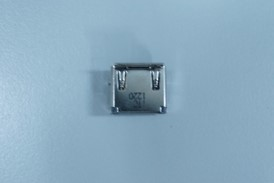
\includegraphics[width=1in,height=0.6in]{j_img/wp11.jpg} & 
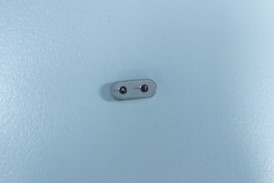
\includegraphics[width=1in,height=0.6in]{j_img/wp15.jpg} & 
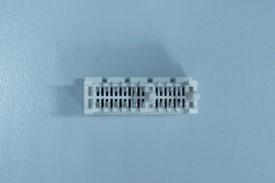
\includegraphics[width=1in,height=0.6in]{j_img/wp21.jpg} & 
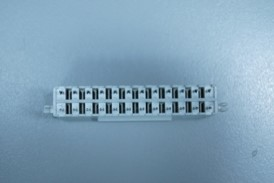
\includegraphics[width=1in,height=0.6in]{j_img/wp25.jpg} &
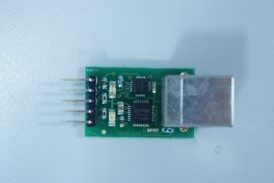
\includegraphics[width=1in,height=0.6in]{j_img/wp31.jpg} & 
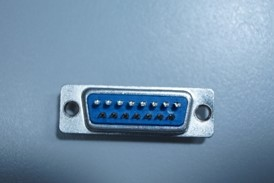
\includegraphics[width=1in,height=0.6in]{j_img/wp35.jpg} \\
\hline
WP1.2 & WP1.6 & WP 2.2 & WP 2.6 & WP3.2 & WP3.6\\
\hline
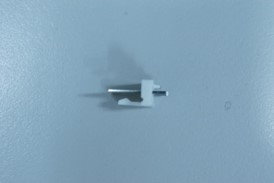
\includegraphics[width=1in,height=0.6in]{j_img/wp12.jpg} & 
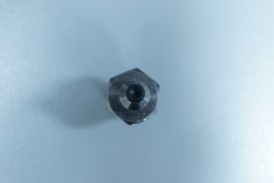
\includegraphics[width=1in,height=0.6in]{j_img/wp16.jpg} & 
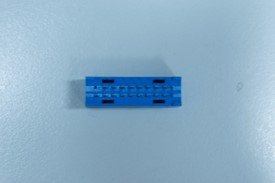
\includegraphics[width=1in,height=0.6in]{j_img/wp22.jpg} & 
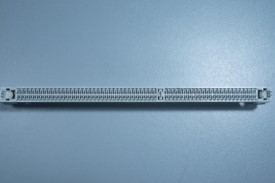
\includegraphics[width=1in,height=0.6in]{j_img/wp26.jpg} &
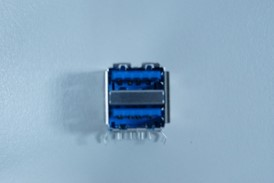
\includegraphics[width=1in,height=0.6in]{j_img/wp32.jpg} & 
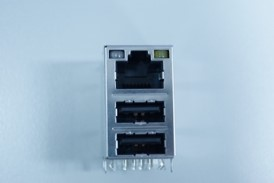
\includegraphics[width=1in,height=0.6in]{j_img/wp36.jpg} 
\\
\hline
WP1.3 & WP1.7 & WP 2.3 & & WP3.3 & WP3.7\\
\hline
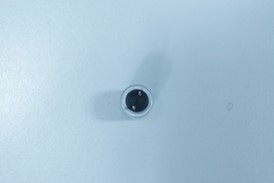
\includegraphics[width=1in,height=0.6in]{j_img/wp13.jpg} & 
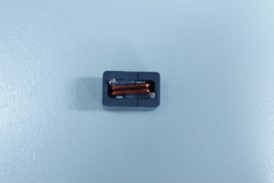
\includegraphics[width=1in,height=0.6in]{j_img/wp17.jpg} & 
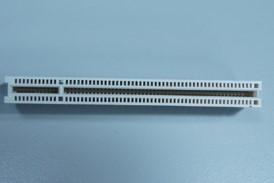
\includegraphics[width=1in,height=0.6in]{j_img/wp23.jpg} & 
 &
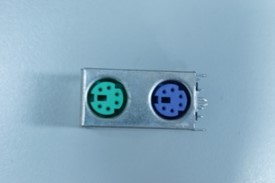
\includegraphics[width=1in,height=0.6in]{j_img/wp33.jpg} & 
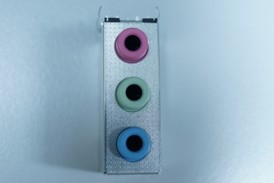
\includegraphics[width=1in,height=0.6in]{j_img/wp37.jpg} 
\\
\hline
WP1.4 & & WP 2.4 & & WP3.4 &\\
\hline
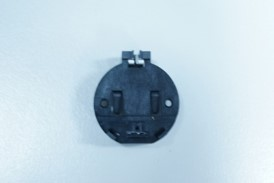
\includegraphics[width=1in,height=0.6in]{j_img/wp14.jpg} & 
 & 
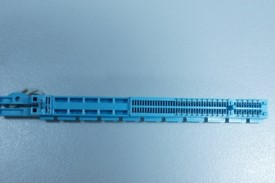
\includegraphics[width=1in,height=0.6in]{j_img/wp24.jpg} & 
 &
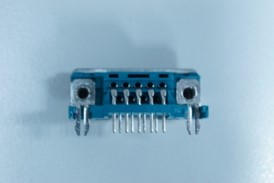
\includegraphics[width=1in,height=0.6in]{j_img/wp34.jpg} & 
\\ 
\hline
\end{tabular}
\end{center}
\end{table*}

The testing work pieces are classified into three classes in table 2. For class $\bf{WP1}$, the work pieces are featureless and small, so it's hard to construct robustness descriptor even building relational model for entire model. For class $\bf{WP2}$, all work pieces acquire similar shapes or size, so, for general method, this kind of object is easily mismatch in the matching process. The work pieces in $\bf{WP3}$ are matched group of this experiment. The work pieces acquire sufficient feature for descriptor, and have plenty of information for identifying and constructing relational model. In the first stage of experiment, we would like to compare the performance of proposed system between different classes in different environments.  The results of different classes are shown in fig.6. In fig.6(b), the environment lighting is controlled by on-axis lighting source, so the information of object are more complete and distinct than images with lighting control in fig.6(a). The accuracy of recognized result is average of 100 times repeatedly testing.

 The system is considered convergence while accuracy is over 95$\%$, and stop learning approach. If the accuracy is under 95$\%$ again, the learning approach would be re-excuted. Comparing the results, in both cases, class $\bf{WP3}$ could be convergent with least input sample, and convergent time of class $\bf{WP2}$ is slowest. The results shows the efficiency of learning could be slightly improved by environment constrain, but the accuracy is not effected, and always over 95$\%$ after learning approach stopped. Similarly, twenty kinds of work pieces are included in learning stage in the same time, and the results are shown in fig. 7. The accuracy of each test is also the average of 100 times repeatedly testing. The results show that system need more inputs to convergent while more kinds of objects are included in learning stage. The performance is also slightly improved while environment is lighting controlled. In brief, these two experiments verify proposed system is competent to learn the relational model automatically. Although the learning rate would be dragged by the kinds of input objects, the learning rate still can be convergent by reasonable number of inputs. The result shows the system can be convergent by less than 1000 sample pieces with random poses. Furthermore, the accuracy of recognition is stable once learning approach completing, and would not be under threshold(95$\%$) again unless adding new kind input.


 
\begin{figure}[!t]
\centering
	\subfigure[Performance without environment constrains]{
		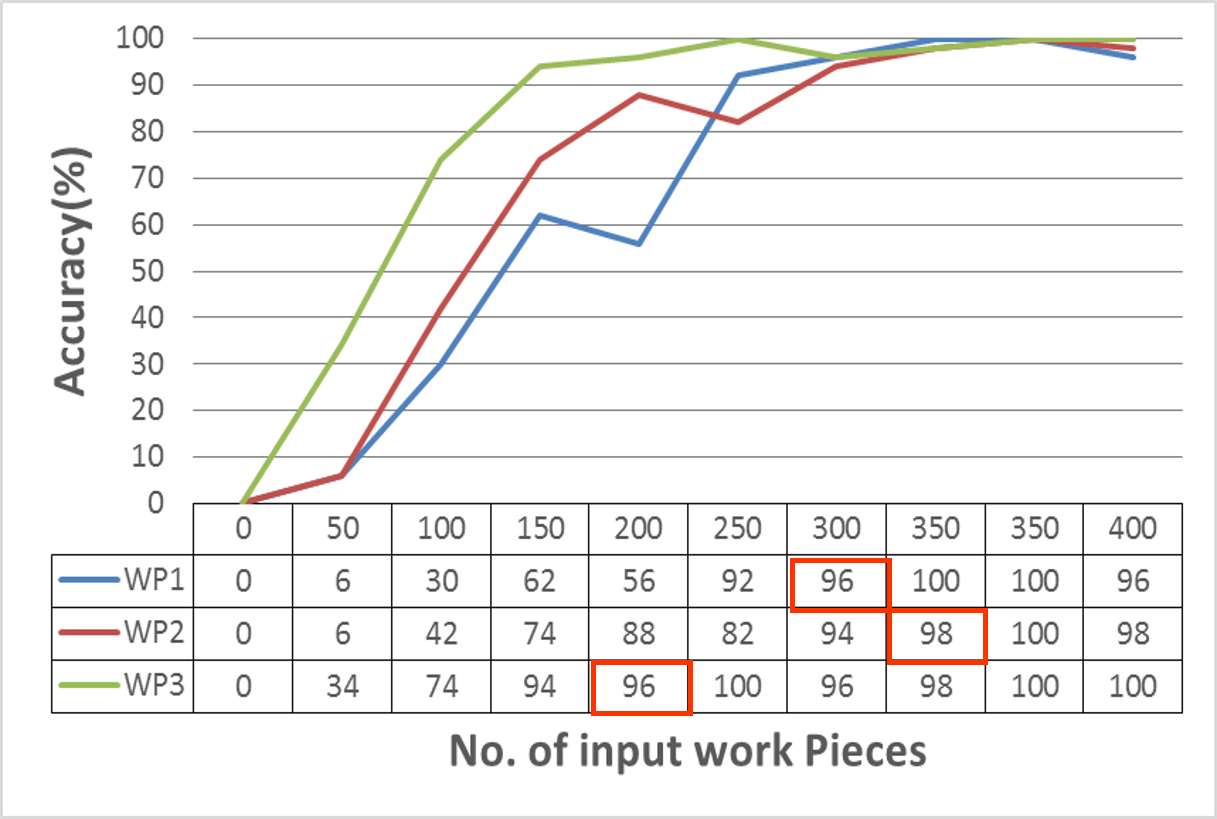
\includegraphics[width=3 in]{j_img/exp02.png}
	}

	\subfigure[Performance with environment constrains]{
		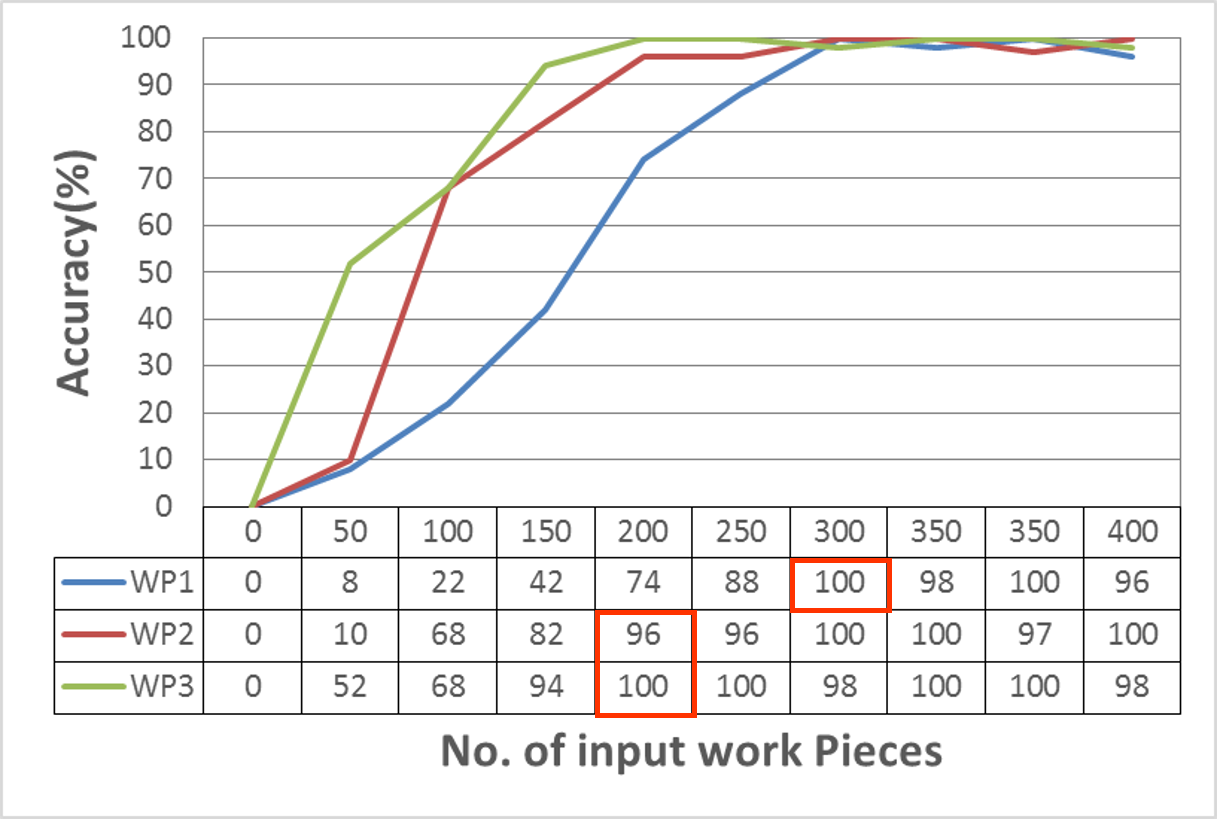
\includegraphics[width=3 in]{j_img/exp01.png}
	}

\caption{Experimental Results of different classes in different environment constrains}

\end{figure}

\begin{figure}[!t]
\centering
	\subfigure[Performance without environment constrains]{
		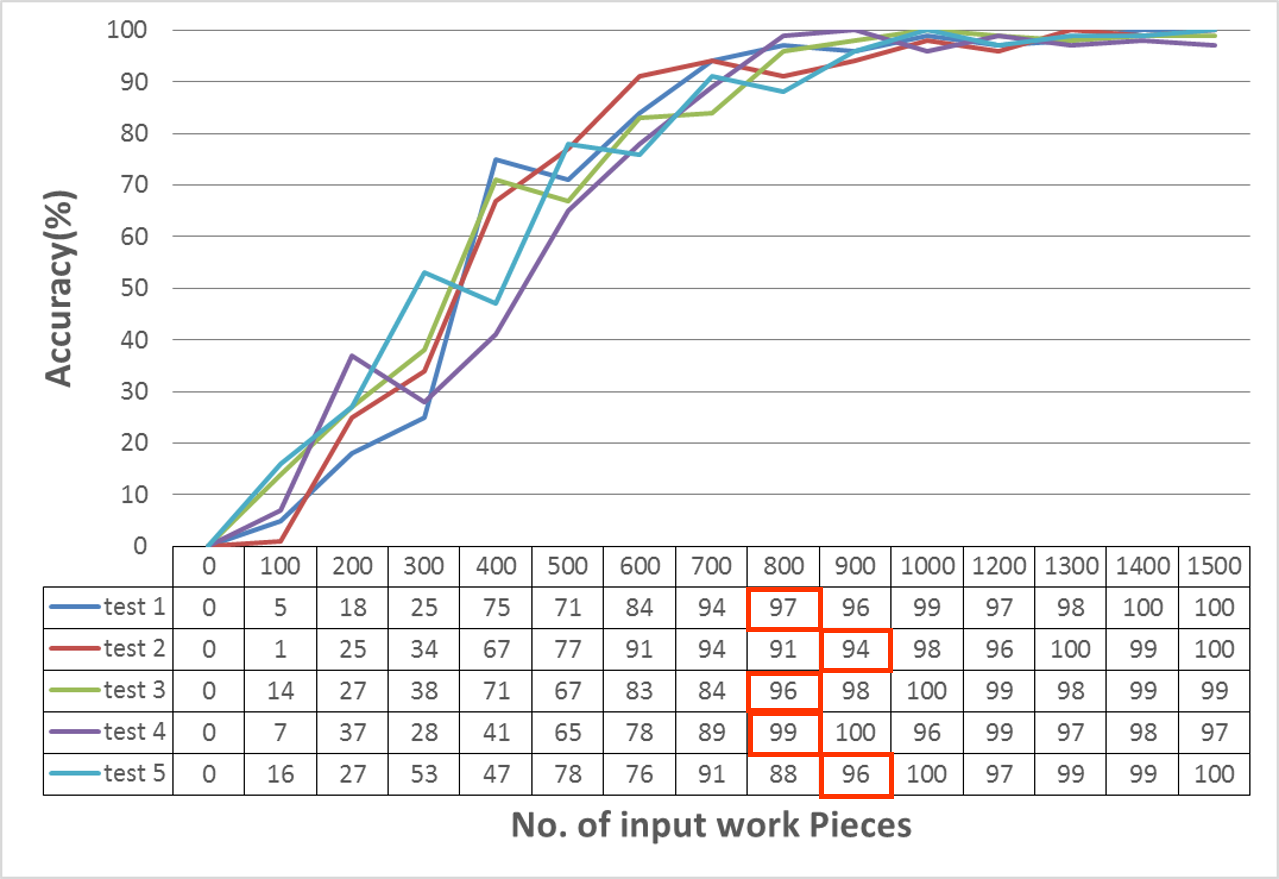
\includegraphics[width=3 in]{j_img/exp04.png}
	}

	\subfigure[Performance with environment constrains]{
		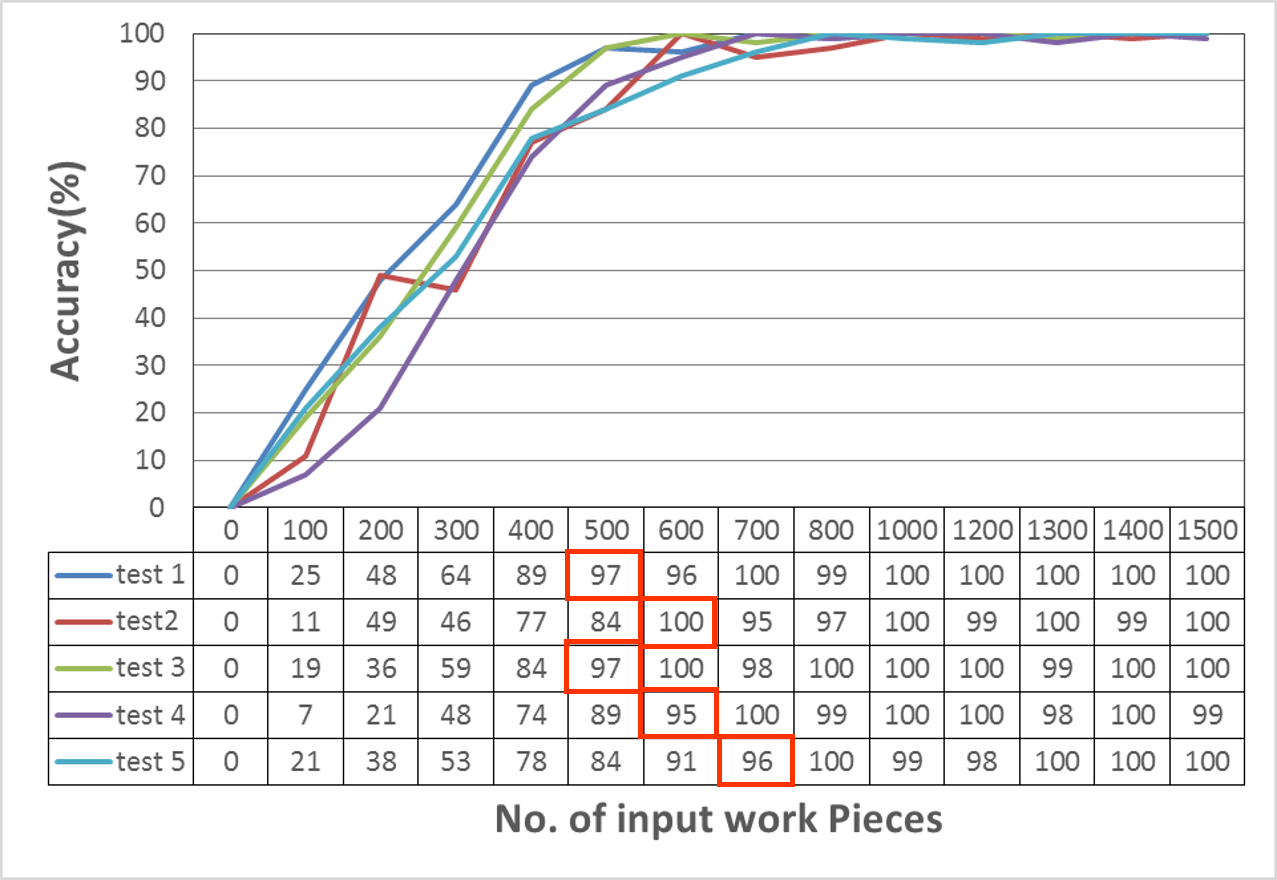
\includegraphics[width=3 in]{j_img/exp03.png}
	}

\caption{Experimental Results of all work pieces in different environment constrains}

\end{figure}

The experiment in fig. 6 and 7 testified the performance of proposed system could automatically learn the relational model of variant kinds of objects. Then, we would like to compare the performance of proposed system with other advanced approaches. Since none of similar systems could handle this issue in our survey, so the comparisons would be done by dividing our system into two parts. One is 2-D descriptors for each face of objects, and the other is machine learning approach for learning relational model.

For the descriptor part, four kinds of other descriptors are chosen to compare with proposed system. B-SIFT[25]and Edge-SIFT[26] are modified versions of SIFT approach which enhanced the accuracy of feature point registration. BRISK[13] descriptor is constructed based on binary robust invariant scalable key points, and Zernike Moment (ZM)[11] phase-based descriptor is a moment-based descriptor which use the phase information of signal. All of these descriptors are representative methods in relative field recent years, and had been testified by plenty of researchers. To compare the robustness and accuracy, the performance is testified by two conditions. One is relationship of each faces is prior of system, and the descriptors only provide information for object matching. The experiments are implemented by the same learning approach which proposed in previous section.The other is no prior for learning approach that information of descriptor need to use for inferring the relational model. The ZM descriptor have the best performance in the condition without prior, but accuracies of descriptors are close. In condition without prior, the MLN-based descriptor acquire best performance which testified MLN-based descriptor is suited for automatic learning system. 

Hereafter, the performance of different learning methods should be further discussed. The learning approach in proposed system need to learn the distribution of different domains, so regular learning approaches is hard to applied on proposed structure directly. The transfer learning methods are famous for handling cross domains problem, so the other three kinds of transfer learning approaches: Locally Weighted Ensemble approach(LWE)[7], Transductive SVM(TSVM)[8], and Weighted Neural Network(WNN)[9] are chosen to compare with proposed method. Similarly, the experiments are divided into two parts as shown in table 4. The result shows LEW had the best accuracy in the condition with prior, and proposed learning approaches acquire greatest performance in condition without prior, but, in both two conditions, the performance between different methods are pretty close. It's seem the results are mainly effected by the performance of the descriptor. The performance of descriptor not only influence the result of 2-D image, but also the relational model of each faces, so the experiments are reasonable. Furthermore, the results showed proposed system acquire best performance in automatic learning part.  

\newcommand{\tabincell}[2]{\begin{tabular}{@{}#1@{}}#2\end{tabular}}

\begin{table}[!t]
\caption{Comparisons of system performance with different 2-D descriptors}
\centering
\begin{tabular}{|c|c|c|c|c|c|c|} 
\hline
\multirow{2}{*}{} &
&
\multicolumn{5}{|c|}{\bf{Descriptor}} \\
\cline{3-7}
 &
 & 
\bf{\tabincell{l}{MLN-\\based}} &
\bf{B-SIFT} &
\bf{\tabincell{l}{Edge-\\SIFT}} &
\bf{BRISK} &
\bf{ZM} 
 \\
\hline
\multirow{4}{*}{\tabincell{l}{With\\prior}} &
WP1 &
0.9781&
0.9664&
0.8384&
0.9556&
0.9788
\\
\cline{2-7}
&
WP2 &
0.9630&
0.9766&
0.9233&
0.9676&
0.9523
\\
\cline{2-7}
&
WP3 &
0.9901&
0.9963&
0.9454&
0.9899&
0.9949
\\
\cline{2-7}
&
All &
0.9594&
0.8982&
0.8066&
0.9432&
0.9634
\\
\hline\hline
\multirow{4}{*}{\tabincell{l}{Without\\prior}} &
WP1 &
0.9611&
0.7688&
0.6544&
0.8103&
0.7787
\\
\cline{2-7}
&
WP2 &
0.9505&
0.7043&
0.7123&
0.7197&
0.7979
\\
\cline{2-7}
&
WP3 &
0.9718&
0.8044&
0.7963&
0.8243&
0.8231
\\
\cline{2-7}
&
All &
0.9543&
0.6431&
0.6144&
0.7741&
0.7670
\\
\hline

\end{tabular} 
\end{table} 

\begin{table}[!t]
\caption{Comparisons of different transfer learning approach}
\centering
\begin{tabular}{|l|l|l|l|l|l|} 
\hline
\multirow{2}{*}{} &
&
\multicolumn{4}{|c|}{\bf{Transfer learning approach}} \\
\cline{3-6}
 &
 & 
\bf{Proposed} &
\bf{LEW} &
\bf{TSVM} &
\bf{WNN} 
\\
\hline
\multirow{4}{*}{\tabincell{l}{With\\prior}} &
WP1 &
0.9781&
0.9802&
0.9511&
0.9513
\\
\cline{2-6}
&
WP2 &
0.9630&
0.9763&
0.9690&
0.9601
\\
\cline{2-6}
&
WP3 &
0.9901&
0.9899&
0.9799&
0.9684
\\
\cline{2-6}
&
All &
0.9594&
0.9677&
0.9567&
0.9541
\\
\hline\hline
\multirow{4}{*}{\tabincell{l}{Without\\prior}} &
WP1 &
0.9611&
0.9601&
0.9543&
0.9103
\\
\cline{2-6}
&
WP2 &
0.9505&
0.9543&
0.9558&
0.9197
\\
\cline{2-6}
&
WP3 &
0.9718&
0.9788&
0.9699&
0.9346
\\
\cline{2-6}
&
All &
0.9603&
0.9553&
0.9497&
0.9486
\\
\hline

\end{tabular} 
\end{table} 




\section{Conclusion}
The automatic learning approaches for visual-servo system is an important part in industrial application. In this work, we reverse the concept of traditional visual-servo system. The robustness of feature points and descriptor is not the thing which should be most concerned. Instead, the relational model between input and output is the most important. 

To learn the relationship between input and output, we proposed a system architecture which can automatic learning and self-supervised the performance of learning or inference results. Since the relationship between input and output is consisted by multiple different domains, the relational model is further segmented into three domain:2-D descriptor, 3-D object and Cartesian space of robot arm. Instead of modelling by three independent networks, these three domains are integrated into one multi-layers networks. Comparing with traditional multi-layers percetron, proposed multi-layer networks is not used to model a complex non-linear distribution, but model the transfer function between different layers. 
The knowledge in different domains could be transfer between different layers through transfer functions which are called relational models in this paper.  Furthermore, a MLN-based descriptor is further proposed to assist inference relationship of each 2-D descriptor while the relational model is unknown. The experiments result shows the system could automatic learning the relational model, and performance could compete with other excellent methods.  





.
\ifCLASSOPTIONcaptionsoff
  \newpage
\fi




\begin{thebibliography}{1}

\bibitem{IEEEhowto:kopka}
Torgny Brogårdh, \emph{"Present and future robot control development—An industrial perspective"},\hskip 1em plus
  0.5em minus 0.4em\relax Annual Reviews in Control, Volume 31, Issue 1, pp. 69–79, 2007.

\bibitem{IEEEhowto:kopka} 
Ebrahim Mattar, \emph{"Robotics Arm Visual Servo: Estimation of Arm-Space Kinematics Relations with Epipolar Geometry, Robotic Systems - Applications, Control and Programming"},\hskip 1em plus
  0.5em minus 0.4em\relax Dr. Ashish Dutta (Ed.), ISBN: 978-953-307-941-7, InTech, DOI: 10.5772/25605.

\bibitem{IEEEhowto:kopka} 
So-Youn Park ,Yeoun-Jae Kim ,Ju-Jang Lee ,Byung Soo Kim, and Khalid A.Alsaif,\emph{"Controlling robot arm manipulator using image-based visual servoing without pre-depth information"},\hskip 1em plus 0.5em minus 0.4em\relax  37th IEEE Interantional Conferece on Industrial Electronics, pp.3157-3161,Nov. 2011.

\bibitem{IEEEhowto:kopka} 
K. Deguchi, H. Sakurai, and S. Ushida,\emph{"A Goal Oriented just-in-time visual servoing for ball catching robot arm”},\hskip 1em plus 0.5em minus 0.4em\relax in Int. Conf. on Intelligent Robots and Systems, Sept. 2008, pp. 3034–3039.
Sa\v{s}o D\v{z}eroski\emph{"Multi-relational Data Mining: An Introduction"},\hskip 1em plus 0.5em minus 0.4em\relax SIGKDD Explore Newsletter, Volume 5, Issue 1, July 2003, pp.1-16.

\bibitem{IEEEhowto:kopka} 
Sinno Jialin Pan, and  Qiang Yang,\emph{"A Survey on Transfer Learning"},\hskip 1em plus 0.5em minus 0.4em\relax Knowledge and Data Engineering, IEEE Transactions on , vol.22, no.10, pp.1345,1359, Oct. 2010


\bibitem{IEEEhowto:kopka} 
T. Dietterich, L. Getoor, and K. Murphy,\emph{"Statistical Relational Learning and its Connections to Other Fields"},\hskip 1em plus 0.5em minus 0.4em\relax ICML-2004 Workshop on Statistical Relational Learning (SRL), Banff, Canada, July 2004.

\bibitem{IEEEhowto:kopka} 
Jing Gao and Wei Fan and Jing Jiang and Jiawei Han, \emph{"Knowledge Transfer via Multiple Model Local Structure Mapping"},\hskip 1em plus 0.5em minus 0.4em\relax in the 14th ACM SIGKDD International Conference on Knowledge Discovery and Data Mining,pp. 283-291,New York, USA,2008

\bibitem{IEEEhowto:kopka} 
T. Joachims, \emph{"Making large-scale svm learning practical."},\hskip 1em plus 0.5em minus 0.4em\relax advances in kernel methods - support vector learning, MIT-Press, 1999.
D. Lowe, \emph{"Distinctive Image Features from Scale-Invariant Keypoints"},\hskip 1em plus 0.5em minus 0.4em\relax International Journal of Computer Vision 60(2), pp. 91–110, 2004.

\bibitem{IEEEhowto:kopka} 
A. J. Carlson, C. M. Cumby, J. L. R. Nicholas D. Rizzolo,
and D. Roth,\emph{"Snow learning architecture"},\hskip 1em plus 0.5em minus 0.4em\relax Technical report UIUCDCS, 1999.

\bibitem{IEEEhowto:kopka} 
H. Bay, A. Ess, T. Tuytelaars, and L. Gool,\emph{"SURF: Speeded up robust features"},\hskip 1em plus 0.5em minus 0.4em\relax Comput. Vis. Image Understand., vol. 110, no. 3, pp. 346–359, Mar. 2008.

\bibitem{IEEEhowto:kopka} 
Zen Chen and Shu-Kuo Sun,\emph{"A Zernike Moment Phase-Based Descriptor for Local
Image Representation and Matching"},\hskip 1em plus 0.5em minus 0.4em\relax IEEE Trans. Image
Process., vol. 19, no. 1,pp. 205–219, Jan. 2010.

\bibitem{IEEEhowto:kopka} 
A. Alahi, R. Ortiz, and P. Vandergheynst,\emph{"Freak: Fast retina keypoint"},\hskip 1em plus 0.5em minus 0.4em\relax CVPR, 2012.

\bibitem{IEEEhowto:kopka} 
S. Leutenegger, M. Chli, and R. Siegwart,\emph{"Brisk: Binary Robust Invariant Scalable Keypoints"},\hskip 1em plus 0.5em minus 0.4em\relax International conference on Computer Vision, 2011.

\bibitem{IEEEhowto:kopka} 
 Vijay Chandrasekhar, Gabriel Takacs, David Chen, Sam S. Tsai, Jatinder Singh, and Bernd Girod,\emph{"Transform coding of image feature descriptors,"},\hskip 1em plus 0.5em minus 0.4em\relax SPIE 7257, Visual Communications and Image Processing, 2009.

\bibitem{IEEEhowto:kopka} 
Matthew Richardson and Pedro Domingos,\emph{"Markov logic networks,"},\hskip 1em plus 0.5em minus 0.4em\relax International Journal of Machine Learning, Volume 62, Issue 1-2,pp 107-136, Feb. 2006.

\bibitem{IEEEhowto:kopka} 
L. Mihalkova, T. Huynh, and R.J. Mooney,\emph{“Mapping and
Revising Markov Logic Networks for Transfer Learning”,},\hskip 1em plus 0.5em minus 0.4em\relax Proc. 22nd Assoc. for the Advancement of Artificial Intelligence (AAAI) Conf. Artificial Intelligence, pp 608-614, July 2007.

\bibitem{IEEEhowto:kopka} 
Kok, Stanley and Domingos, Pedro,\emph{"Learning the Structure of Markov Logic Networks"},\hskip 1em plus 0.5em minus 0.4em\relax Proceedings of the 22Nd International Conference on Machine Learning, pp 441-448, Germany, 2005.

\bibitem{IEEEhowto:kopka} 
Parag Singla and Pedro Domingos,\emph{"Discriminative training of Markov logic networks"},\hskip 1em plus 0.5em minus 0.4em\relax Proceedings of the international Conf. on Artificial Intelligence, 2005.

\bibitem{IEEEhowto:kopka} 
J. Shi and J. Malik,\emph{"Normalized cuts and image segmentation"},\hskip 1em plus 0.5em minus 0.4em\relax Pattern Analysis and Machine Intelligence, IEEE Transactions on , vol.22, no.8, pp.888,905, Aug 2000.

\bibitem{IEEEhowto:kopka} 
Karthikeyan Vaiapury, Anil  Aksay and Ebroul Izquierdo,\emph{"GrabcutD: Improved Grabcut Using Depth Information"},\hskip 1em plus 0.5em minus 0.4em\relax Proceedings of the 2010 ACM Workshop on Surreal Media and Virtual Cloning, pp 57-62, New York, USA, 2010.

\bibitem{IEEEhowto:kopka} 
Z. Zivkovic,\emph{"Improved adaptive Gaussian mixture model for background subtraction"},\hskip 1em plus 0.5em minus 0.4em\relax Pattern Recognition, 2004. ICPR 2004. Proceedings of the 17th International Conference on , vol.2, no., pp.28,31 Vol.2, 23-26 Aug. 2004.

\bibitem{IEEEhowto:kopka} 
G. Frahling and C. Sohler,\emph{"A fast k-means implementation using coresets"},\hskip 1em plus 0.5em minus 0.4em\relax  Proceedings of the twenty-second annual symposium on Computational geometry (SoCG),2006.

\bibitem{IEEEhowto:kopka} 
Tong Simon, and Daphne Koller,\emph{"Support vector machine active learning with applications to text classification"},\hskip 1em plus 0.5em minus 0.4em\relax  The Journal of Machine Learning Research 2 pp 45-66, 2002.

\bibitem{IEEEhowto:kopka} 
Fei Sha and Fernando Pereira,\emph{"Shallow parsing with conditional
random fields"},\hskip 1em plus 0.5em minus 0.4em\relax Proceedings of the 2003 Conference of the North American Chapter of the Association for Computational Linguistics on Human Language Technology, Volume 1, 2003.

\bibitem{IEEEhowto:kopka} 
Yanning Zhang,Zhi-Hua Zhou, Changshui Zhang and Li, Ying,\emph{"B-SIFT: A Highly Efficient Binary SIFT Descriptor for Invariant Feature Correspondence"},\hskip 1em plus 0.5em minus 0.4em\relax Intelligent Science and Intelligent Data Engineering, pp 426-433, 2012

\bibitem{IEEEhowto:kopka} 
S. Zhang, Q. Tian, K. Lu, Q. Huang and W. Gao,\emph{"Edge-SIFT: Discriminative binary descriptor for scalable partial-duplicate mobile search"},\hskip 1em plus 0.5em minus 0.4em\relax ” IEEE Trans. Image Process., vol. 22, no. 7, pp. 2889–2902, Jul. 2013.












\end{thebibliography}


\end{document}


